\chapter{Herramientas y tecnologías utilizadas}
\label{cap:herramientas}

	\chapterquote{Siempre llega una nueva herramienta. La tecnología es neutral, depende de cómo se use}{Rick Smolan}

En este capítulo hablaremos sobre las distintas herramientas y tecnologías utilizadas para el desarrollo del trabajo. También expondremos los motivos por los cuales hemos decidimos usar unas tecnologías frente a otras.


\section{Flask}\label{sec:flask}


Flask\footnote{\href{https://openwebinars.net/blog/que-es-flask/}{https://openwebinars.net/blog/que-es-flask/}} es un ``micro'' framework minimalista escrito en Python con la finalidad de facilitar el desarrollo de aplicaciones web y APIs. Desarrollado por Armin Ronacher a partir de 2010, actualmente es uno de los frameworks más populares para implementar en Python. Este framework\footnote{\href{https://leanmind.es/es/desarrollo/backend/python/}{https://leanmind.es/es/desarrollo/backend/python/}} está basado en la especificación WSGI de Werkzeug y el motor de templates Jinja2 y tiene una licencia BSD (licencia utilizada para los sistemas operativos, y que tiene menos restricciones en comparación con otras licencias como la GPL). 

El término ``micro'' hace referencia a que Flask trae únicamente por defecto las herramientas necesarias para crear una aplicación web básica. Si éstas no fueran suficientes hay un conjunto muy grande de extensiones (plugins) que se pueden instalar fácilmente proporcionando así libertad a los desarrolladores ya que contiene muy poco código predefinido.

Algunas de las características de Flask por las que decidimos desarrollar nuestra aplicación web con este framework son las siguientes:

\begin{itemize}
	\item Agilidad, rapidez y facilidad en la instalación y configuración, que a diferencia de otros framework como Django, son más complejos y difíciles de usar.
	\item Compatible con Python.
	\item Incluye un servidor web de desarrollo. No es necesaria una infraestructura con un servidor web para probar las aplicaciones, sino que de forma sencilla se puede levantar un servidor web e ir viendo los resultados que se van obteniendo.
	\item Cuenta con un depurador. Si en algún momento obtenemos un error en el código que se está desarrollando, se puede depurar ese error y ver los valores de las variables.
	\item Buen manejo de rutas. Se controlan todas las peticiones que hacen los clientes y se tienen que determinar que ruta está accediendo el cliente para ejecutar el código necesario.
	\item Cuenta con documentación extensa para el desarrollo de aplicaciones.
\end{itemize}

%\begin{figure}[h!]
%	\centering
%	
%	
%	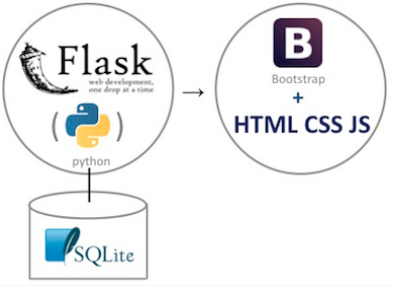
\includegraphics[scale=0.9]{Imagenes/Figuras/Flask}
%	
%	
%	\caption{Framework Flask.}
%	\label{fig:entornoFlask}
%\end{figure}


\section{spaCy}\label{sec:spacy}

El Procesamiento del Lenguaje Natural (PLN)\footnote{\href{https://www.iic.uam.es/inteligencia/que-es-procesamiento-del-lenguaje-natural/ }{https://www.iic.uam.es/inteligencia/que-es-procesamiento-del-lenguaje-natural/ }} es el campo de conocimiento de la Inteligencia Artificial y la lingüística que intenta replicar la facultad del lenguaje humano, es decir, comunica las máquinas con las personas mediante el uso de lenguas naturales, como el español, el inglés o el chino.

Existe una amplia variedad de herramientas informáticas para el PLN en diversos idiomas, como NLTK, spaCy, Scikit-learn, entre otras. En nuestro caso hemos decidido usar spaCy por su fácil uso, rapidez y precisión a la hora de realizar análisis sintácticos.

spaCy\footnote{Para más información acceder a \href{https://spacy.io/}{https://spacy.io/}} es una librería de código abierto que permite construir aplicaciones de PLN escrita en Python. Actualmente es considerada una de las mejores herramientas para el PLN. 


Esta librería contiene los datos lingüísticos y los algoritmos que necesitará para procesar textos en lenguaje natural. Proporciona objetos que ayudan a representar elementos de texto, como oraciones y palabras. Estos objetos tienen una serie de atributos que representan las características lingüísticas. Además, nos ofrece visualizadores integrados para generar un gráfico de la estructura sintáctica de una oración. Puede ser usada para extraer informacion, para sistemas de comprensión del lenguaje natural o para el pre-procesado de texto para deep learning.

spaCy es capaz de realizar las siguientes tareas PLN:

\begin{itemize}
	\item \textbf{Tokenization}: Divide una oración en tokens, donde cada token	representa cada una de las palabras que componen dicha oración.
	\item \textbf{Part-of-speech (POS) Tagging}: asigna a cada token una etiqueta gramatical, designando su categoría gramatical (sustantivo o nombre, adjetivo, pronombre, verbo, etc.).
	\item \textbf{Dependency Parsing}: analiza una oración para establecer la dependencia gramatical de las palabras ``principales'' y otras que modifican las principales, describiendo la relación entre ellas. El resultado del análisis es la creación de un árbol de dependencias, así como el etiquetado de dependencia en cada palabra como muestra la Figura \ref{fig:dependeciaSpacy}. 
	\begin{figure}[h!]
		\centering
		
		
		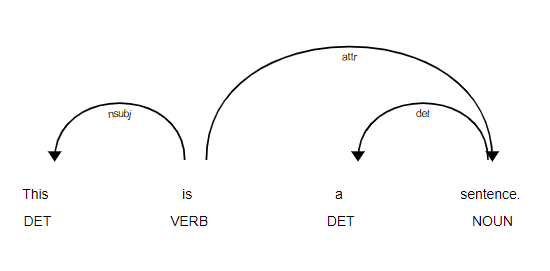
\includegraphics[scale=1]{Imagenes/Figuras/dependenciaSpacy}
		
		
		\caption{Árbol de dependencias.}
		\label{fig:dependeciaSpacy}
	\end{figure}
	
	

	\item \textbf{Lemmatization}: : permite obtener el lema correspondiente de una
	palabra. Por ejemplo, el lema de ``dije'' es ``decir'' y el de ``ratas'' es ``rata''.
	\item \textbf{Sentence Boundary Detection}: detecta el límite de una oración.
	\item \textbf{Named Entity Recognition}: busca, ubica y clasifica palabras en el texto en categorías predefinidas como los nombres de personas, organizaciones, ubicaciones, fechas, etc. 
	\item \textbf{Entity Linking}: desambiguado de entidades textuales a identificadores únicos en una base del conocimiento.
	\item \textbf{Similarity}: compara palabras, intervalos de texto y documentos para saber qué grado de similitud tienen entre ellos.
	\item \textbf{Text Classification}: asigna categorías o etiquetas a un documento completo, o a partes de un documento.
	\item \textbf{Rule-based Matching}: busca secuencias de tokens basada en sus textos y anotaciones lingüísticas, similar a expresiones regulares.

\end{itemize}

\section{NIL-WS-API}\label{sec:nilws}

NIL-WS-API\footnote{Para más información acceder a \href{https://holstein.fdi.ucm.es/nil-ws-api/}{https://holstein.fdi.ucm.es/nil-ws-api/}} en una API del grupo NIL (Interacción natural basada en el lenguaje) implementada en el proyecto IDiLyCo, según el estándar OpenAPI 3.0.1. 

El grupo NIL\footnote{\href{http://nil.fdi.ucm.es/}{http://nil.fdi.ucm.es/}} surge en 2005 de un grupo de investigadores y profesionales cuyo objetivo principal es el desarrollo de tecnologías basadas en el lenguaje natural, para poder usarse en aplicaciones prácticas y ser aplicadas en la vida real. 

Está API ofrece una gran cantidad de servicios a nuestra disposición. Entre ellos podemos encontrar servicios para:


\begin{itemize}
	\item Palabras: servicios que devuelven información relativa a una palabra.
	\item Textos: servicios que devuelven información relativa  un texto a o un grupo de palabras.
	\item Pictogramas: servicios que devuelven información relativa a un pictograma.
	\item Simplificación de texto: servicios para la simplificación léxica.
	\item Resúmenes: ofrece una simplificación sintáctica a partir del resumen de un texto.
	\item Emociones: servicios para obtener las emociones de una palabra, una frase o un texto. 
\end{itemize}

De todos estos servicios, para nuestro asistente hemos hecho uso de los que se refieren a las palabras (algunos de ellos se muestran en la Figura \ref{fig:apiNILWS}), que detallaremos en el capítulo \ref{cap:implementacion}, sección \ref{sec:serviciosWebExternos}.

	\begin{figure}[h!]
	\centering
	
	
	\includegraphics[scale=0.7]{Imagenes/Figuras/apiNil}
	
	
	\caption{Algunos de los servicios que ofrece NIL-WS-API referidas a palabras.}
	\label{fig:apiNILWS}
\end{figure}
\section{Postman}\label{sec:postman}

Postman\footnote{\href{https://openwebinars.net/blog/que-es-postman/}{https://openwebinars.net/blog/que-es-postman/}} surgió originariamente como una extensión para el navegador Google Chrome. Se trata de una herramienta dirigida a desarrolladores web que permite realizar peticiones HTTP a cualquier API. Es muy útil a la hora de programar y hacer pruebas, para comprobar el correcto funcionamiento de nuestros desarrollos.

Además de hacer peticiones a servicios, que es su objetivo principal, nos ofrece un conjunto de funcionalidades que nos ayudarán a organizar las peticiones en colecciones, hacer y automatizar pruebas, mantener equipos sincronizados y crear Mocks de APIs.

Es una herramienta gratuita en su versión básica pero además ofrece dos posibilidades de pago que mejoran las características.
	\begin{figure}[h!]
	\centering
	
	
	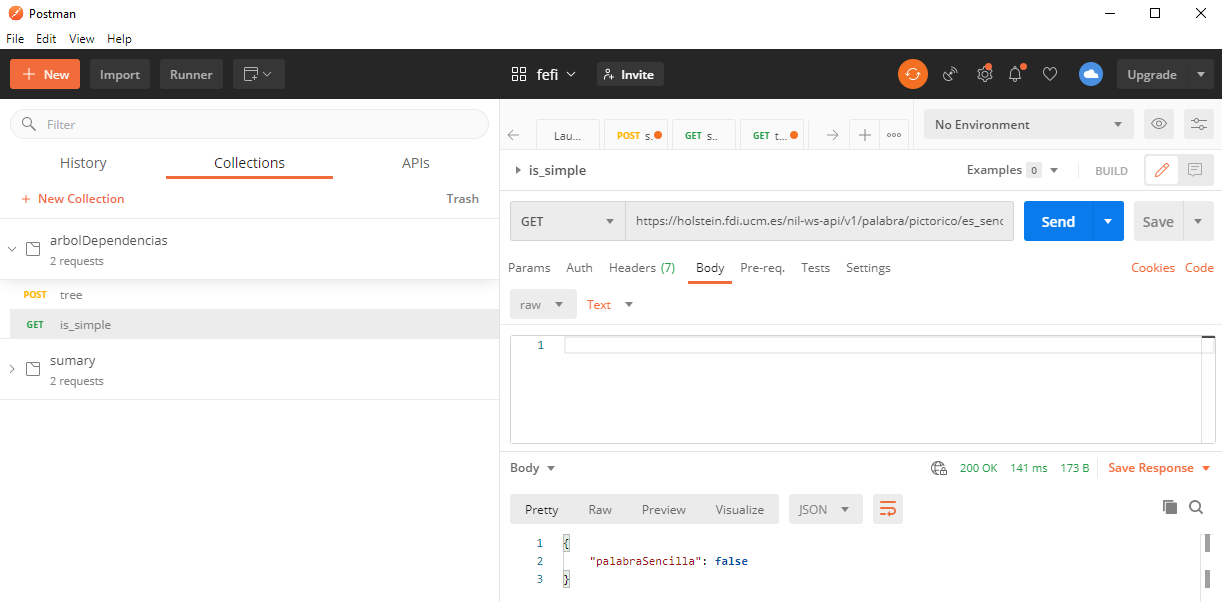
\includegraphics[scale=0.6]{Imagenes/Figuras/postman}
	
	
	\caption{Petición hecha con Postman}
	\label{fig:postman}
\end{figure}

En nuestro caso, hemos usado esta herramienta para probar todos los endpoints y APIs, y comprobar que todos los datos recibidos eran los correctos o esperados.

\section{PyCharm}

PyCharm\footnote{\href{https://blog.desdelinux.net/pycharm-un-entorno-de-desarrollo-para-python/}{https://blog.desdelinux.net/pycharm-un-entorno-de-desarrollo-para-python/}}, desarrollado por la empresa JetBrains, es un entorno de desarrollo (IDE) para desarrollar principalmente código en Python. Cuenta con un depurador y un intérprete que nos ayudarán a saber o conocer los posibles errores del código en tiempo real. 

Además ofrece un soporte para HTML que incluye sintaxis y resaltado de errores, formateo de acuerdo con el estilo del código, validación de la estructura, finalización del código, etc.

Este IDE lo hemos usado en el desarrollo de la aplicación web (Figura \ref{fig:pycharm})
	\begin{figure}[h!]
	\centering
	
	
	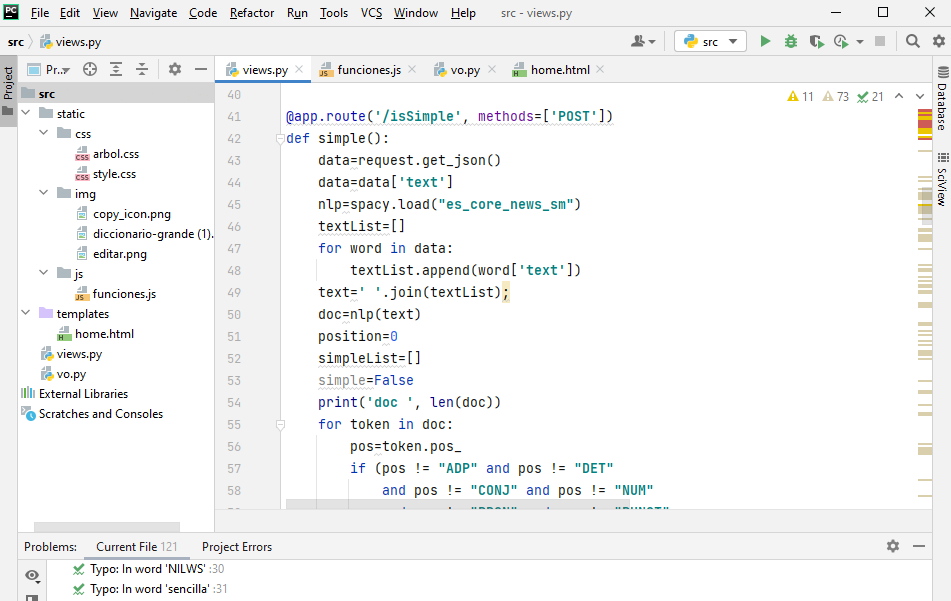
\includegraphics[scale=0.5]{Imagenes/Figuras/pycharm}
	
	
	\caption{IDE PyCharm}
	\label{fig:pycharm}
\end{figure}